\chapter{The likelihood formalism}\label{app:likelihood}

\section{Definition}

Throughout the analysis, parameter estimation is performed under the likelihood formalism, whereby the maximum likelihood estimator for a set of $m$ parameters $\bm{\theta}$, $L(\bm{\theta})$, is maximised
%
\begin{equation}
    \frac{\partial \ln L(\bm{\theta})}{\partial \theta_j} = 0\ ,
\end{equation}
%
where $j$ enumerates the set $\bm{\theta}$ from $1$ to $m$. For a set of $n$ statistically independent measurements $\bm{x}$, each sampled from a probability density function $f(x_i;\bm{\theta})$ given the set of parameters, the likelihood function is
%
\begin{equation}
    L(\bm{\theta}) = \prod_{i=1}^{n}f(x_i;\bm{\theta})\ .
\end{equation}
%
The set of parameters which maximises this functions is denoted $\hat{\bm{\theta}}$.

For large sample size, typical with \CMS data, the maximisation procedure become computationally demanding. Instead, the data is binned and the measurements $\bm{x}$ represent the event count in the bins. Typically the event count in a particular bin is considered to be a random variable, hence the probability density function is a poisson distribution $P$ for the binned data, given a prediction $\bm{\nu}$,
%
\begin{equation}
    f(x_i;\bm{\theta}) = P(x_i;\nu_i(\bm{\theta}))\ .
\end{equation}
%
The poisson distribution is replaced by a multinomial distribution if the event count is considered as fixed. The predictions $\bm{\nu}$ are determined from a functional form or estimated from MC simulations.

The set of parameters may contain unconstrained parameters such as a signal strength multiplier as well as constrained parameters, known as nuisances parameters, which encode systematic uncertainties. For the estimation of a signal strength multiplier the parameters are divided into unconstrained $\bm{\mu}$, gaussian constrained $\bm{\theta}$ and poisson constrained $\bm{\phi}$ characterising limited MC sample sizes \cite{Barlow:1993dm}. With these parameters the likelihood function is given by
%
\begin{equation}
    L(\bm{\mu},\bm{\theta},\bm{\phi}) = \prod_{i=1}^{n}P(x_i;\nu_i(\bm{\mu},\bm{\theta},\phi_i))P(n_i;\gamma_i(\phi_i))\prod_{j=1}^{m}N(\theta_j)\ ,
\end{equation}
%
where $N(\theta_j)$ is a gaussian distribution with a zero mean and unit width, $P(n_i;\gamma_i(\phi_i))$ is a poisson distribution extended to real numbers for weighted MC events with an effective number of entries $n_i$ (the ratio of the sum of weighted events to its variance) with a $\phi_i$ dependent prediction $\gamma_i$. This prediction is given by
%
\begin{equation}\label{eq:gammai}
    \gamma_i(\phi_i) = n_i\left(1 + \frac{1}{\sqrt{n_i}}\right)^{\phi_i}
\end{equation}
%
to allow $\phi_i$ to taken any real number value without resulting in a negative prediction. The factor $1 + 1/\sqrt{n_i}$ is chosen to yield convenient values for $\phi_i$, typically between $-1$ and $+1$. The poisson constraints are applied to each bin on the overall MC prediction, summing all signal and background contributions. For a single signal and single background process, with contributions $s_i$ and $b_i$, the prediction $\nu_i$ takes the form
%
\begin{equation}
    \nu_i(\mu,\bm{\theta},\phi_i) = \frac{\gamma_i(\phi_i)}{n_i}\left(\mu s_i(\bm{\theta}) + b_i(\bm{\theta})\right)
\end{equation}
%
The $\bm{\theta}$ dependence of $s_i(\bm{\theta})$ and $b_i(\bm{\theta})$ is determined from alternative MC templates generated at $\theta_k=-1,0,+1$, with all other values interpolated or extrapolated \cite{Conway:2011in}. To encode the shape dependence of these nuisance parameters along a particular dimension the set of bins $i=1$ to $n$ are split into $N$ categories, each with $M$ bins along the `shape' dimension. The effect of the nuisance parameters is factorised into the inclusive normalisation $r_{\mathrm{norm}}$ and a shape morphing term $r_{\mathrm{morph}}$:
\begin{equation}
    s_{i,j}(\bm{\theta}) = s_{i,j}\prod_{k=1}^{m}r_{\mathrm{norm},i,k}(\theta_k)\sum_{j=1}^{m}(1+r_{\mathrm{morph},i,j,k}(\theta_k))\ ,
\end{equation}
where the signal contribution is subscripted by the categorisation $i$ and shape dimension bin $j$ with MC prediction for the signal $s_{i,j}$, and a similarly defined relationship for the background $b_{i,j}(\bm{\theta})$. The normalisation term is determined from the MC templates generated at ${\theta_k=-1,0,+1}$: $s_{i,j,k}^{-}$, $s_{i,j}$ and $s_{i,j,k}^{+}$; as
%
\begin{equation}
    r_{\mathrm{norm},i,k}(\theta_k) = \left(\frac{1}{\sum_{j=1}^{M}s_{i,j}}\sum_{j=1}^{M}
    \begin{dcases}
        s_{i,j,k}^+ & \text{if }\theta_k> 0\\
        s_{i,j,k}^- & \text{otherwise}
    \end{dcases}\right)^{|\theta_k|}\ .
\end{equation}
%
Meanwhile, the shape morphing term extrapolates linearly for $|\theta_k|>1$ with a smooth polynomial below this range:
%
\begin{equation}
    r_{\mathrm{morph},i,j,k} = \frac{\theta_k}{2\hat{s}_{i,j}}\left(\Delta_{i,j,k} + \Sigma_{i,j,k}p(\theta_k)\right)\ ,
\end{equation}
%
where the hat denotes parameters normalised by their sum across the shape dimension, and the other parameters are defined as
%
\begin{align}
    \Delta_{i,j,k} & = \hat{s}_{i,j,k}^+ - \hat{s}_{i,j,k}^-\ ,\\
    \Sigma_{i,j,k} & = (\hat{s}_{i,j,k}^+-\hat{s}_{i,j}) + (\hat{s}_{i,j,k}^{-}-\hat{s}_{i,j})\ ,\\
    p(\theta_k) & =
    \begin{dcases}
        \frac{1}{8}\theta_k\left(\theta_k^2(3\theta_k^2-10)+15\right) & \text{if }|\theta_k|< 1 \\
        \theta_k/|\theta_k| & \text{otherwise}\ .
    \end{dcases}
\end{align}
%
This procedure is known as vertical template morphing\cite{Conway:2011in} which uses normalised parameters to avoid double-counting the normalisation effects, with a linear dependence on $\theta_k$ for symmetric uncertainties and a smooth, differentiable polynomial to alter asymmetric uncertainties. A similar dependence is defined for all other processes.


\section{Limited sample size of alternative templates}\label{appsec:alt_temp_smooth}

The accuracy of the vertical template morphing procedure is highly dependent on the quality of the alternative MC templates $s_{i,j,k}^+$ and $s_{i,j,k}^-$ which may suffer from the limited sample size in MC. Although the statistical size of the nominal template $s_{i,j}$ is incorporated in the likelihood, the alternative MC templates are assumed to be precisely known. This issue typically exists for background processes with a small cross section compared to a larger process, hence should not have a substantial impact on the parameters of interest. However, an alternative template with a small sample size which results in an abnormally large systematic effect in a particular bin will lead to a significant constraint on the associated nuisance parameter. If this systematic uncertainty is correlated with one of the larger processes then the impact of this systematic uncertainty may be severely underestimated on the parameter of interest.

To avoid issues with the limited sample size of alternative templates, additional constrained nuisance parameters are introduced in each bin for each systematic uncertainty, to allow the fit to effectively smooth out fluctuations due to the limited sample size. However, this would introduce a significant number of parameters to fit, beyond the computational power available. Instead the alternative templates are smoothed prior to the fitting procedure, as required. The procedure involves regularising large statistical variations in the relative $\pm 1\sigma$ variation templates. Bins centres are interpolated with a smoothing spline, where each point is inversely weighted by it's uncertainty, with a subsequent gaussian smearing to prevent large changes between adjacent bins. The normalisation effect of the variations is fixed during this smearing procedure. An example of the smoothing procedure is shown in Fig.~\ref{fig:smoothing_example}. This method proves to reduce the constraint on systematic uncertainties with a limited sample size, leading to an overall increase in the uncertainty on the parameter of interest. The smoothing procedure is only used where it is required, ensuring the method does not lead to a significant loss in information.

\begin{figure}
    \centering
    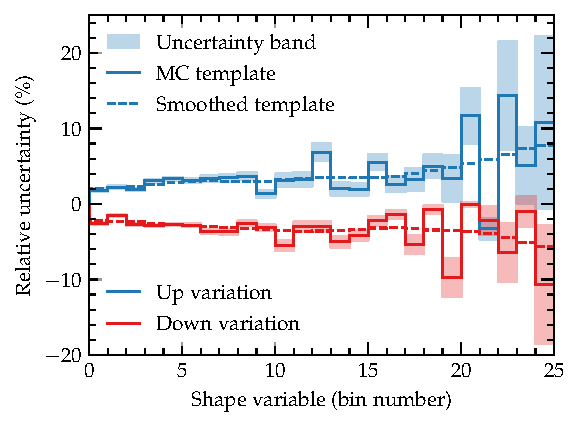
\includegraphics{appendices/100_appendices/images/smoothing_example.pdf}
    \caption[Example of MC alternative template smoothing.]{
        Smoothing of a statistically limited MC alternative template by a spline followed by a gaussian smear. The uncertainty band represents the uncorrelated uncertainty between the up and down variation as a representative uncertainty. The resulting smoothed template has significantly reduced the variation between adjacent bins, especially in the final bins where the statistical uncertainty is the greatest.
    }
    \label{fig:smoothing_example}
\end{figure}

%Bins are smeared within gaussian distributions to minimise the difference between adjacent bins, within the MC statistical uncertainty of each bin.


\section{Alternative templates}\label{appsec:alt_temp}

The nuisance parameters affect the normalisation and shape of the \recoil distribution by interpolating between and extrapolating from alternative templates on the MC, shown in Figs.~\ref{fig:alt_templates_bkg} and \ref{fig:alt_templates_sig} for the \IVj processes. As detailed in Sec.~\ref{appsec:alt_temp_smooth}, these templates are smoothed in situations where the MC sample size is too small. Some of these templates cancel in the transfer factor for $r_{\mathrm{inv}}$ measurement, such as the theory uncertainties. However, the JES, JER and unclustered energy uncertainties are evidently limited by the MC sample size. Although smoothing aids at determined the `true' template, it cannot reproduce an underlying correlation such as for the JES uncertainty between various processes. Therefore, the {$2$--$\SI{5}{\%}$} JES uncertainty on the \IZvvj process in the \metplusjets region may be consistent with all other processes, however, the limited MC sample size limits our knowledge of this. This results in non-cancellation of uncertainties, such as JES, which are expected to cancel in ratios of the various \IVj processes.

\begin{figure}[htb]
    \centering
    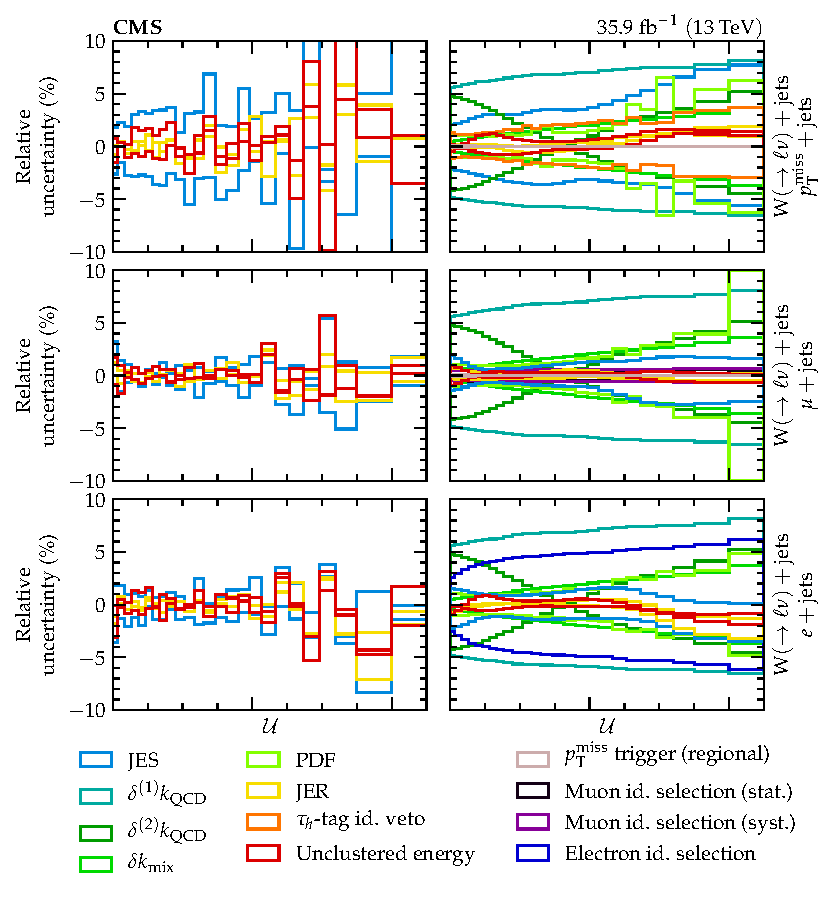
\includegraphics{appendices/100_appendices/images/alt_templates_bkg.pdf}
    \caption{
        The 12 most significant alternative templates on the \IWj process. The left column shows the template prior to smoothing while the right column shows the same template after smoothing. Templates which only appear in the right column are not smoothed.
    }
    \label{fig:alt_templates_bkg}
\end{figure}

\begin{figure}[htb]
    \centering
    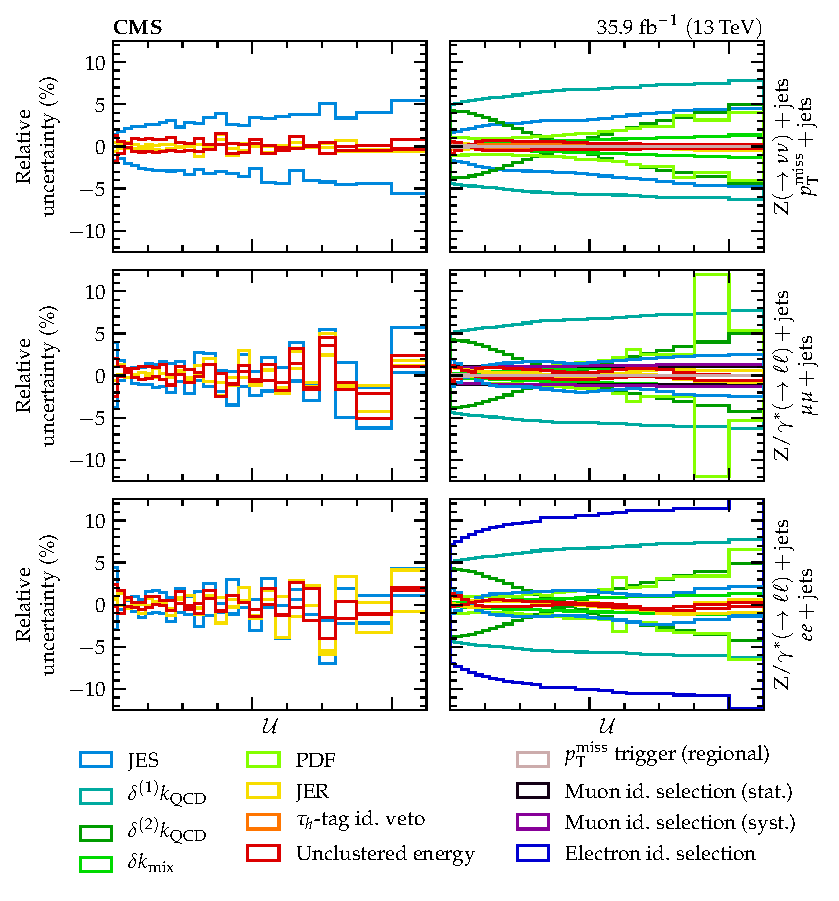
\includegraphics{appendices/100_appendices/images/alt_templates_sig.pdf}
    \caption{
        The 12 most significant alternative templates on the \IVj processes within the signal region. The left column shows the template prior to smoothing while the right column shows the same template after smoothing. Templates which only appear in the right column are not smoothed.
    }
    \label{fig:alt_templates_sig}
\end{figure}